% V2 (short): set-point and gain modification only, under 5 pages.
% Based on the IEEE conference template (IEEEtran, conference mode), with small deviations
% (author block with advisors, tighter floats); the 8-page version is main_v2_long.tex.
\documentclass[conference]{IEEEtran}
\IEEEoverridecommandlockouts
\usepackage{cite}
\usepackage{amsmath,amssymb,amsfonts}
\usepackage{graphicx}
\usepackage{textcomp}
\usepackage{xcolor}
\usepackage{booktabs}
\usepackage{url}
\usepackage{tikz}
\usetikzlibrary{arrows.meta,positioning,calc}

\newcommand{\R}{\mathbb{R}}
\newcommand{\T}{^{\top}}
\newcommand{\mpc}{\mathrm{MPC}}
\newcommand{\xb}{\bar{x}}
\newcommand{\ub}{\bar{u}}
\setlength{\textfloatsep}{8pt plus 2pt minus 2pt}
\setlength{\dbltextfloatsep}{8pt plus 2pt minus 2pt}
\setlength{\abovecaptionskip}{3pt}

\begin{document}

\title{Control Policy Refiner in Legged Robotics:\\ Direction and Preliminary Results}

\author{\IEEEauthorblockN{Norawit Nangsue\textsuperscript{1,2}}
\IEEEauthorblockA{Advisors: Fumio Kanehiro\textsuperscript{1,2} and Mehdi Benallegue\textsuperscript{1}}
\IEEEauthorblockA{\textsuperscript{1}CNRS-AIST JRL (Joint Robotics Laboratory), IRL,\\
National Institute of Advanced Industrial Science and Technology (AIST), Japan\\
\textsuperscript{2}University of Tsukuba, Ibaraki, Japan}}

\maketitle

\begin{abstract}
Model predictive control (MPC) gives a humanoid robot a motion that respects its dynamics, but only as well as its model allows; reinforcement learning (RL) improves from experience, but an unstructured learned correction ignores what the MPC already knows.
A whole-body MPC based on differential dynamic programming returns a feedback policy, made of a state set-point and a gain matrix, that drives the robot between two solves.
We propose a \emph{control policy refiner}: an RL policy that shifts this set-point and modifies these gains, so that the torque correction is produced by the MPC's own feedback law.
We give low-dimensional parametrizations of both that are consistent with the contacts and with the solver's local model.
As the base controller, we implemented an IS-MPC gait generator with a reformulated footstep timing and position pre-optimization and a whole-body MPC of the HRP-5P legs.
In MuJoCo it walks at up to 0.3\,m/s with a mean whole-body solve time of 6.7\,ms and recovers from 26 of 36 pushes.
The refiner itself has not been trained yet.
\end{abstract}

\begin{IEEEkeywords}
humanoid robots, model predictive control, residual reinforcement learning, feedback gains
\end{IEEEkeywords}

\section{Introduction}

Two families of controllers make humanoid robots walk.
Model-based controllers plan with a reduced model such as the linear inverted pendulum (LIPM) \cite{kajita2001lipm} and track the plan with a whole-body controller, increasingly a whole-body MPC \cite{mastalli2020crocoddyl,dantec2022wbmpc}.
Learning-based controllers train a neural network policy in simulation with RL \cite{radosavovic2024humanoid}.
An MPC handles constraints explicitly and can be re-targeted without retraining, but it is optimal only for its model, which leaves out joint flexibility, contact compliance and actuator dynamics.
An RL policy absorbs such effects from experience, but it is a black box whose behaviour is fixed at training time.

Residual RL \cite{johannink2019residual} keeps the model-based controller and learns only a correction, so that exploration starts from a working behaviour.
Recent legged-robot results combine the two in this way or by tracking a model-based plan \cite{jenelten2024dtc,jeon2025residualmpc}.
The correction is usually added to the controller output as a joint torque or position target.
It is then unstructured: one free number per joint at every control step, in actuator coordinates, with nothing tying it to the model that produced the base action.

A whole-body MPC solved by differential dynamic programming (DDP) \cite{mayne1966ddp} offers a more structured place.
The solver returns Riccati gains with the torque trajectory.
Together they form a feedback policy with a \emph{set-point} (the planned state) and a \emph{reactiveness} (the gains), which is the law that drives the robot between two solves \cite{grandia2019feedback,dantec2022firstorder}.
In existing work these gains are applied as computed.
Learning gains instead of outputs is known from variable impedance control \cite{buchli2011variable}; we apply it online to the time-varying gains of a humanoid whole-body MPC and combine it with a shift of the set-point.

This report gives the direction of the work and its first results:
(i) a formulation of the refiner on the DDP feedback policy, with parametrizations of the set-point shift and of the gain modification (Section~\ref{sec:method});
(ii) the base controller it will refine (Section~\ref{sec:base});
(iii) simulation results of the base controller that show what the refiner has to correct (Section~\ref{sec:results}).

\section{Base Controller}
\label{sec:base}

\begin{figure*}[t]
\centering
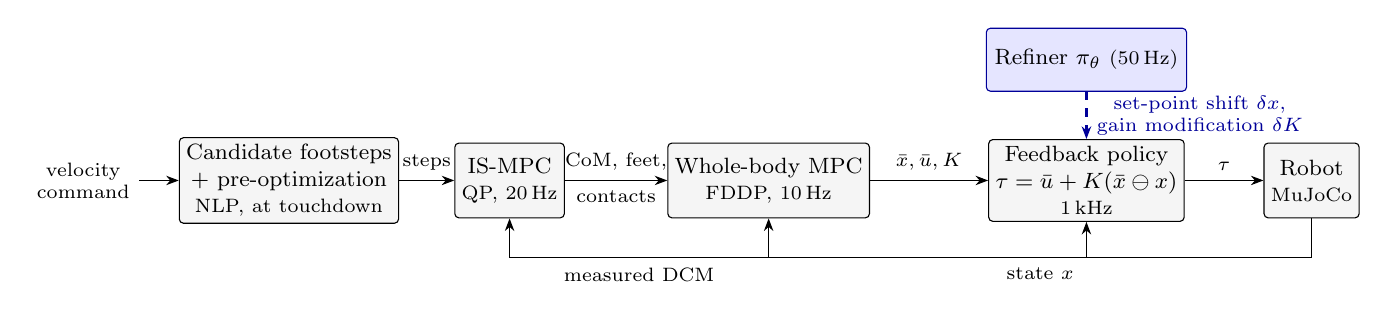
\begin{tikzpicture}[font=\footnotesize, >={Stealth[length=1.6mm]},
  blk/.style={draw, rounded corners=1.5pt, minimum height=9.5mm, align=center, inner sep=2.5pt, fill=black!4},
  res/.style={draw, rounded corners=1.5pt, minimum height=8mm, align=center, inner sep=3pt, fill=blue!10, draw=blue!60!black},
  lab/.style={font=\scriptsize, align=center},
  inj/.style={->, dashed, blue!60!black, thick}]
\node[lab] (cmd) {velocity\\command};
\node[blk, right=5mm of cmd] (ftpp) {Candidate footsteps\\+ pre-optimization\\{\scriptsize NLP, at touchdown}};
\node[blk, right=7mm of ftpp] (ismpc) {IS-MPC\\{\scriptsize QP, 20\,Hz}};
\node[blk, right=13mm of ismpc] (wb) {Whole-body MPC\\{\scriptsize FDDP, 10\,Hz}};
\node[blk, right=15mm of wb] (ric) {Feedback policy\\$\tau=\ub+K(\xb\ominus x)$\\{\scriptsize 1\,kHz}};
\node[blk, right=10mm of ric] (rob) {Robot\\{\scriptsize MuJoCo}};
\draw[->] (cmd) -- (ftpp);
\draw[->] (ftpp) -- node[lab, above] {steps} (ismpc);
\draw[->] (ismpc) -- node[lab, above] {CoM, feet,} node[lab, below] {contacts} (wb);
\draw[->] (wb) -- node[lab, above] {$\xb,\ub,K$} (ric);
\draw[->] (ric) -- node[lab, above] {$\tau$} (rob);
\coordinate (fb) at ($(rob.south)+(0,-5mm)$);
\draw[->] (rob.south) -- (fb) -| node[lab, pos=0.25, below] {state $x$} (wb.south);
\draw[->] (fb -| ric.south) -- (ric.south);
\draw[->] (fb -| wb.south) -| node[lab, pos=0.25, below] {measured DCM} (ismpc.south);
\node[res, above=6mm of ric] (pol) {Refiner $\pi_\theta$ {\scriptsize (50\,Hz)}};
\draw[inj] (pol.south) -- node[lab, right, text=blue!60!black] {set-point shift $\delta x$,\\gain modification $\delta K$} (ric.north);
\end{tikzpicture}
\caption{Base controller (grey, implemented) and the proposed refiner (blue, dashed, not yet trained). The refiner shifts the set-point $\xb$ and modifies the Riccati gains $K$ of the feedback policy returned by the whole-body MPC; it never outputs a torque directly.}
\label{fig:arch}
\end{figure*}

Fig.~\ref{fig:arch} shows the controller: a LIPM gait generator at 20\,Hz, a whole-body MPC of the legs at 10\,Hz, and its feedback policy at 1\,kHz.

\subsection{Gait generator}
With CoM $c$, ZMP $p$ and $\eta=\sqrt{g/z_c}$, the divergent component of motion (DCM) $\xi=c+\dot c/\eta$ obeys $\dot\xi=\eta(\xi-p)$.
It stays bounded if and only if \cite{lanari2014boundedness}
\begin{equation}
\xi(t_0)=\eta\int_{0}^{\infty}e^{-\eta\tau}\,p(t_0+\tau)\,d\tau .
\label{eq:stab}
\end{equation}
IS-MPC \cite{scianca2020ismpc} enforces \eqref{eq:stab} as a constraint of a QP on the ZMP velocity and the footsteps, with the ZMP kept inside the support region.
After a push, \eqref{eq:stab} may be infeasible with the nominal step times, so the footstep positions $p_f^k$ and times $t_k$ are first adjusted by a pre-optimization \cite{dallard2025adios}: integrating \eqref{eq:stab} piecewise over the steps requires the DCM to lie in a sum of the support regions weighted by $\mu_k-\mu_{k+1}$, with $\mu_k=e^{-\eta t_k}$.

This problem is badly scaled, since $\mu_k$ reaches $10^{-7}$ at the end of the preview, and the reference implementation \cite{ismpcwalking} solves it by block coordinate descent between positions and times, dropping the divisor of the displacement term.
We replace $\mu_k$ by the ratio $\nu_k=\mu_k/\hat\mu_k$ to its nominal value, which makes all variables of order one, keep the original cost
\begin{multline}
J=\sum_k(\nu_k-1)^2+w_s\|s\|^2\\
+K_s\sum_{i\ge1}\big\|p_f^i-\hat p_f^i\big\|^2\,
\frac{(\nu_i\hat\mu_i-\nu_{i-1}\hat\mu_{i-1})^2}{(\hat\mu_i-\hat\mu_{i-1})^2},
\label{eq:cost}
\end{multline}
where $s$ is the slack of the DCM condition, and solve positions and times jointly as one nonlinear program with CasADi \cite{andersson2019casadi} and IPOPT \cite{wachter2006ipopt}.
The IS-MPC QP then uses the result as candidates, with a 2.5\,s control horizon, an anticipative tail up to 6\,s and a term that centres the ZMP in the sole, and is solved with OSQP \cite{stellato2020osqp}.
The generator replans at every touchdown and re-solves the QP every 50\,ms.
It includes capture steps and a DCM feedback law for standing, and detects a push when the measured DCM jumps by more than 4\,cm from the planned one within a tick.

\subsection{Whole-body MPC and its feedback policy}
The whole-body problem uses the floating base and the twelve leg joints of HRP-5P \cite{kaneko2019hrp5p} ($n_v=18$), with rigid 6D contacts that follow the gait generator's schedule and a cost that tracks its CoM and foot references.
It has 25 nodes of 20\,ms and is solved with the FDDP solver of Crocoddyl \cite{mastalli2020crocoddyl} every 100\,ms, with at most ten warm-started iterations.
Each solve returns the state and torque trajectories $\xb_i,\ub_i$ and the Riccati gains $K_i$.
Between solves, the torque is
\begin{equation}
\tau^{\mpc}=\ub_i+K_i\,(\xb_i\ominus x),
\label{eq:riccati}
\end{equation}
evaluated at 1\,kHz with the measured state $x$; $\ominus$ is the difference on the state manifold.

\section{Control Policy Refiner}
\label{sec:method}

\subsection{The feedback policy as the interface}
In \eqref{eq:riccati}, the set-point $\xb$ says where the robot should be, and the gain $K$ says how strongly, and through which joints, it reacts when it is not there.
With the state ordered as base pose, joint positions, base velocity and joint velocities,
\begin{equation}
K=\begin{bmatrix}K_{b}&K_{j}&K_{\dot b}&K_{\dot j}\end{bmatrix}\in\R^{12\times36}.
\label{eq:kpart}
\end{equation}
$K_j$ and $K_{\dot j}$ act as a coupled joint stiffness and damping.
$K_b$ and $K_{\dot b}$ have no equivalent in a joint-space controller: they map an error of the unactuated base to coordinated leg torques through the contact model.
Each solution is executed for 100 control steps, so this law alone determines the behaviour in that interval.
It is optimal for the model.
On the real system, the set-point can be a state the robot should not be driven to, and the gains can be too stiff or too soft for dynamics the model ignores.
The refiner $\pi_\theta$ adjusts these two quantities:
\begin{align}
\tau&=\ub+(K+\delta K)\,\big((\xb\oplus\delta x)\ominus x\big)\nonumber\\
&\approx\tau^{\mpc}+K\,\delta x+\delta K\,e+\delta K\,\delta x,
\label{eq:l2}
\end{align}
with $e=\xb\ominus x$ the tracking error.
It acts at the node rate, 50\,Hz.
A zero output gives exactly the base controller, and the network is initialized to output zero, so training starts from the behaviour of Section~\ref{sec:results}.

\subsection{Set-point modification}
The term $K\delta x$ is a torque restricted to the range of $K$.
The Riccati policy is the first-order expansion of the MPC solution with respect to the state \cite{dantec2022firstorder}, so $K\delta x$ is, to first order, the torque change the MPC itself would command if the robot were displaced by $-\delta x$.
The refiner thus acts as a learned bias on the state seen by the controller, and the result respects the trade-offs of the cost, the dynamics and the contact model.
The action is in state coordinates: through $K_b$ the refiner can ask to move the pelvis toward the stance foot, and the gain distributes this over both legs, a mapping that a torque residual would have to learn for every contact phase.
The shift also enters a loop that is already closed.
With $\zeta_i=x_i\ominus\xb_i$ and $A_i,B_i$ the dynamics Jacobians,
\begin{equation}
\zeta_{i+1}=(A_i-B_iK_i)\,\zeta_i+B_iK_i\,\delta x_i ,
\label{eq:cl}
\end{equation}
so a bounded shift gives a bounded deviation as long as the Riccati gains stabilize the local model.

A free $\delta x$ has 36 components, and a shift that moves a stance foot only creates internal forces.
We restrict it to configurations that keep the stance feet in place:
\begin{equation}
\delta x=\begin{bmatrix}P_c\,S\,a_x\\ 0\end{bmatrix},\qquad P_c=I-J_c^{+}J_c ,
\label{eq:setpoint}
\end{equation}
where $a_x$ is the refiner output, $S$ a selection matrix and $J_c$ the Jacobian of the feet in contact.
With a \emph{base shift} (6 numbers), the refiner outputs a change of the base pose and the projection completes the leg joints; a \emph{full shift} (18 numbers) adds the swing leg.
Both $a_x$ and the resulting torque $K\delta x$ are clipped.

\subsection{Gain modification}
The term $\delta K\,e$ is bilinear: without a tracking error it vanishes, so it changes the reaction to a disturbance and not the nominal motion.
It is the right correction when the motion is right but the reaction is wrong, e.g., gains computed for a rigid contact that are too stiff for a compliant one.
A free $\delta K$ has 432 entries per node and can destabilize the loop.
We consider three parametrizations.

\emph{Output scaling,} $K\leftarrow\mathrm{diag}(e^{a_o})K$, with one scale per joint group (hip, knee, ankle of the stance and of the swing leg).
It sets how much feedback torque each joint contributes.
A continuous-time LQR with a diagonal input weight, as ours, tolerates in each input channel any gain increase and a reduction by half \cite{safonov1977margins}; for a discrete, time-varying gain the margins are smaller, so this indicates a direction and not a guarantee.

\emph{Input scaling,} $K\leftarrow K\,\mathrm{diag}(e^{a_i})$, with one scale per block of \eqref{eq:kpart}.
It sets how much the controller reacts to each kind of error: stiffness against damping, base against joints.

\emph{Cost residual.} The refiner scales a few cost weights, $w\leftarrow w\,e^{a_w}$, and the backward pass is run again along the current trajectory; only its gains are used.
They are optimal for a local problem with positive weights, hence stabilizing for the local model by construction, at the price of one backward pass per decision (a full solver iteration takes about 0.8\,ms).

In all cases the exponential keeps the gains from changing sign, and the scales are rate-limited, because a fast-varying gain can destabilize a loop even when every frozen value is stabilizing.
Table~\ref{tab:param} summarizes the action space.
The refiner cannot change the footsteps, the contact schedule or the feedforward torque: disturbances that need a different step remain the task of the gait generator.

\begin{table}[t]
\caption{Parametrizations of the refiner}
\label{tab:param}
\centering
\setlength{\tabcolsep}{3pt}
\resizebox{\columnwidth}{!}{%
\begin{tabular}{@{}llcl@{}}
\toprule
 & Refiner output & Size & Property\\
\midrule
\multicolumn{4}{@{}l}{\emph{Set-point} ($K\,\delta x$: changes the motion)}\\
Base shift & base pose, legs by projection & 6 & stance feet fixed\\
Full shift & base pose and leg joints & 18 & stance feet fixed\\
\midrule
\multicolumn{4}{@{}l}{\emph{Gain} ($\delta K\,e$: changes the reaction)}\\
Output scaling & scale per joint group & 6 & LQR margins \cite{safonov1977margins}\\
Input scaling & scale per state group & 4 & stiffness vs.\ damping\\
Cost residual & scale per cost weight & 5 & optimal for local model\\
\bottomrule
\end{tabular}}
\end{table}

\subsection{Learning setup}
The refiner observes the state, the tracking error $e$, the feedforward torque, the contact flags and step phase, the velocity command and its previous action.
It is rewarded for velocity tracking and for staying upright, and penalized for the size and rate of its action, for joint torques, for a centre of pressure (CoP) near the sole edge and for a tilted stance foot.
It will be trained with PPO \cite{schulman2017ppo} in simulation with pushes and with mass and friction randomization.

\section{Preliminary Results: Base Controller}
\label{sec:results}

The refiner has not been trained; this section reports the base controller alone.
The HRP-5P model (104\,kg) is simulated in MuJoCo \cite{todorov2012mujoco} with a 1\,ms step and torque control, with $z_c=1.014$\,m and steps of at most 0.8\,s.
Runs are headless on one thread of a laptop (Apple M5).
A fall is a base height below 0.5\,m.
A push is an instantaneous change of the base velocity $\Delta v=\eta d$, which shifts the DCM by $d$ ($d=0.08$\,m is 0.25\,m/s, about 26\,N\,s).

\begin{table}[t]
\caption{Walking in simulation (base controller, no falls)}
\label{tab:walk}
\centering
\setlength{\tabcolsep}{3pt}
\resizebox{\columnwidth}{!}{%
\begin{tabular}{@{}lcccccc@{}}
\toprule
Command & Dist. & Steps & \multicolumn{2}{c}{Error (max) [mm]} & CoP & Solve [ms]\\
 & [m] & & foot & DCM & ratio$^{\mathrm a}$ & mean / max\\
\midrule
0.2\,m/s & 0.93 & 8 & 18 & 28 & 1.45 & 6.4 / 14.2\\
0.3\,m/s, 0.2\,rad/s & 1.46 & 9 & 31 & 40 & 1.81 & 6.9 / 10.0\\
$-0.15$\,m/s & 0.74 & 8 & 10 & 30 & 1.47 & 6.1 / 8.7\\
0.3\,m/s (8\,s) & 2.43 & 13 & 30 & 36 & 1.59 & 7.1 / 11.6\\
\bottomrule
\multicolumn{7}{@{}l}{$^{\mathrm a}$Largest measured CoP offset of a stance foot divided by the half-size}\\
\multicolumn{7}{@{}l}{\phantom{$^{\mathrm a}$}of the largest centred box inside the sole; above 1 is near the sole edge.}
\end{tabular}}
\end{table}

\begin{figure}[t]
\centering
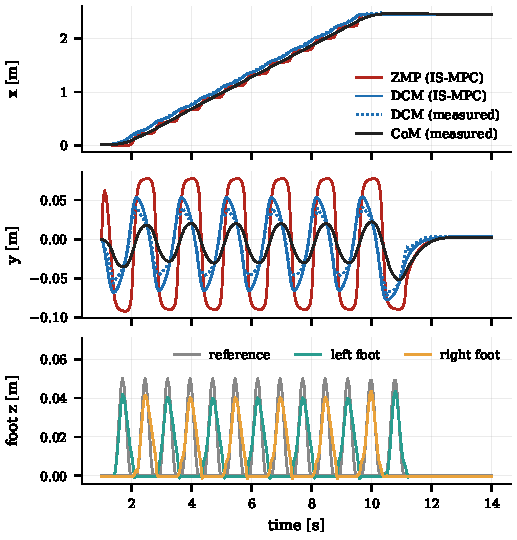
\includegraphics[width=0.8\columnwidth]{figures/walk.pdf}
\caption{Walking at 0.3\,m/s for 8\,s, then stopping: planned ZMP and DCM, measured DCM and CoM (top, middle), and foot heights (bottom).}
\label{fig:walk}
\end{figure}

\begin{table}[t]
\caption{Pushes survived, by DCM shift $d$ (four directions each)}
\label{tab:push}
\centering
\setlength{\tabcolsep}{4pt}
\begin{tabular}{@{}lcccccc@{}}
\toprule
\multicolumn{7}{@{}l}{\emph{Standing}}\\
$d$ [m] & 0.04 & 0.06 & 0.08 & 0.10 & 0.12 & Total\\
\midrule
Push detection on (default) & 4/4 & 4/4 & 4/4 & 1/4$^{\mathrm a}$ & 0/4 & 13/20\\
Push detection off & 4/4 & 4/4 & 2/4 & 1/4 & 0/4 & 11/20\\
\midrule
\multicolumn{7}{@{}l}{\emph{Walking at 0.2\,m/s} (two push instants)}\\
$d$ [m] & \multicolumn{2}{c}{0.05} & \multicolumn{2}{c}{0.08} & & Total\\
\midrule
Default & \multicolumn{2}{c}{7/8} & \multicolumn{2}{c}{6/8} & & 13/16\\
\bottomrule
\multicolumn{7}{@{}l}{$^{\mathrm a}$Two further cases stay up on a tilted foot and are not counted.}
\end{tabular}
\end{table}

\emph{Walking.} The robot does not fall in any of the four commands of Table~\ref{tab:walk} (5\,s each, 8\,s in the last row; Fig.~\ref{fig:walk}).
The measured DCM follows the planned one with an RMS error of 12 to 16\,mm.
The whole-body solve takes 6.7\,ms on average (8.2 iterations) and at most 14.2\,ms of the 100\,ms period; a touchdown replan of the gait generator takes 7.2\,ms on average and the first one 49\,ms.

\emph{Pushes.} Table~\ref{tab:push} reports 20 pushes while standing and 16 while walking.
The robot recovers from 26 of 36.
Closing the loop on the measured DCM helps while standing (all 0.08\,m pushes recovered, against two of four without push detection).
The failures are directional: while walking, the three falls are pushes toward the robot's right; while standing at 0.10\,m, they are the backward and the two lateral pushes.

\emph{What the refiner has to correct.}
(1)~\emph{Contact moments.} The CoP ratio exceeds 1 in every run, and after strong lateral pushes a stance foot rolls onto its edge.
The whole-body problem has no limit on the CoP, so its plan and its feedback ask for ankle moments the sole cannot transmit; a wrench-cone penalty in the cost made walking fail.
A base shift toward the stance foot reduces the moment the plan needs, and a lower output scale on the stance ankle reduces the moment the feedback asks for.
(2)~\emph{Tracking lag.} The robot lags the LIPM reference by 3 to 4\,cm of DCM in single support, systematically and depending on the step phase, which a set-point shift can lead.
(3)~\emph{Reaction to pushes.} The reaction that fails is the one computed by the Riccati gains for the unperturbed plan; whether a stiffer or softer reaction recovers, and in which state groups, is what the gain modification is meant to answer.
Lateral step limits are narrow ($\pm3.5$\,cm), so part of the lateral failures need a different step and are outside the reach of the refiner.

\section{Plan and Conclusion}
\label{sec:plan}

We proposed to refine the control policy of a whole-body MPC by learning on its feedback law: a set-point shift, which becomes the torque the MPC would itself command for a displaced state, and a gain modification, which changes the reaction to errors and leaves the nominal motion unchanged.
The base controller is implemented and walks in simulation, and its weaknesses map to these two parts.

The next step is to train one refiner per row of Table~\ref{tab:param}, then the set-point and gain parts combined, and to compare them on the protocols of Tables~\ref{tab:walk} and~\ref{tab:push} with the base controller and with an unstructured torque residual of the same torque bound.
The MPC runs on the CPU and bounds the training speed: with the measured times, $10^8$ refiner steps at 50\,Hz cost about 60 core-hours of MPC, which is feasible without a GPU-parallel solver \cite{jeon2025residualmpc}.
After simulation, the controller needs a state estimator and a port to mc\_rtc for experiments on HRP-5P.

% slightly smaller, tighter reference list (deviation from the IEEE template to stay within 4 pages)
\begingroup
\renewcommand{\footnotesize}{\fontsize{7.3}{8.3}\selectfont}
\setlength{\itemsep}{0pt}
\bibliographystyle{IEEEtran}
\bibliography{refs}
\endgroup

\end{document}
